\documentclass[10pt,conference]{IEEEtran}
\IEEEoverridecommandlockouts
\usepackage[T1]{fontenc}
\usepackage[utf8]{inputenc}
\usepackage{amsmath,amssymb}
\usepackage{graphicx}
\usepackage{booktabs}
\usepackage{array}
\usepackage{cite}
\PassOptionsToPackage{hyphens}{url}
\usepackage{url}
\usepackage{microtype}
\usepackage[hidelinks]{hyperref}

\DeclareUrlCommand\task{\urlstyle{tt}}
\DeclareUrlCommand\code{\urlstyle{tt}}
% Page budget: let TeX set a paragraph one line shorter whenever it can do so within its normal
% line-breaking tolerance. Fonts, margins and spacing of the IEEE template are untouched.
% Needs the paragraph hooks of LaTeX 2021-06 or later; with an older LaTeX the paper still compiles
% but runs a few lines longer.
\newif\ifsaveline \savelinetrue
\ifdefined\AddToHook
\AddToHook{para/begin}{\ifsaveline\looseness=-1 \fi}
\AddToHook{env/table/begin}{\savelinefalse}
\AddToHook{env/table*/begin}{\savelinefalse}
\fi
% Page budget: the limit is 8 pages. Passages wrapped in \cut{...} are left out of the 8-page build;
% \keepcutstrue prints them again (main_full.tex is this file with that switch on).
\newif\ifkeepcuts \keepcutstrue
\newcommand{\cut}[1]{\ifkeepcuts #1\fi}

\begin{document}

\title{What Does Skill Lift Actually Measure?\\ A Source-Code-Level Audit and\\ Noise-Aware Reanalysis of SkillsBench\thanks{This work has been submitted to the IEEE for possible publication. Copyright may be transferred without notice, after which this version may no longer be accessible.}}

\author{\IEEEauthorblockN{Haozhe Zhang}
\IEEEauthorblockA{Trine University\\
hzhang266@my.trine.edu}
\and
\IEEEauthorblockN{Zhen Long}
\IEEEauthorblockA{National University of Singapore\\
e1351306@u.nus.edu}}

\savelinefalse
\maketitle
\savelinetrue

\begin{abstract}
Agent skills are directories of instructions, reference materials, and scripts loaded on demand by coding agents. According to SkillsBench, although human-curated skills can raise the passing rate by about 16.6 percentage points (pp) on average, they have actually reduced the results for some tasks. Later research has started to gate or eliminate skills according to the above per-task gains. We have audited the above benchmark at the source-code level and analysed 7,554 public trials to form 1,421 paired ``(configuration, task) cells''. Source-code audit identified two controlled-verified cases of grader dependence and one operational definition gap; the average lift on these three tasks was 74.6\,pp, and the overall average lift for the full set was 18.7\,pp. The audit also found that four tasks contained placeholder skill directories, and a certain execution harness additionally added 48 built-in skills in most runs. No task-level reduction achieved statistical significance in the pooled reanalysis with multiple-testing correction. As there were at most three runs per condition for each cell, the observed negative differences are very susceptible to run-sampling noise, and arithmetically, 58\% of the cells could not have shown a decrease. Therefore, the raw numbers of negative cells cannot show that skills cause harm. A gating strategy based on the skill-free score seems to improve by 2-3\,pp in the logs; however, even after shuffling condition labels to remove any skill effect, it still achieves an increase of 4-7\,pp. On the held-out runs not used for fitting and decision-making, there was no statistically significant improvement. The audit ledger and analysis scripts have been published by us.
\end{abstract}

\begin{IEEEkeywords}
agent skills, coding agents, benchmark auditing, evaluation methodology, regression to the mean
\end{IEEEkeywords}

\section{Introduction}
Coding agents such as Claude Code, Codex, Gemini CLI and OpenHands~\cite{wang2025openhands} can achieve specialisation without modifying the model weights by mounting agent skills; some directories contain a \code{SKILL.md} instruction file, as well as optional reference documents and helper scripts. At the start-up, only the short names and descriptions of all the skills are loaded into the context; then, based on relevance assessment by the agent, the entire content of the skill and related files are read~\cite{zhang2025skills}.

SkillsBench~\cite{li2026skillsbench} is the first large-scale benchmark of this mechanism. The fourth one tested 87 containerised tasks in 18 ``model-framework'' configurations under two conditions: with and without human-curated skills mounted; an average pass-rate increase of 16.6\,pp was reported, but there were also considerable variations among configurations and a net decrease in 13 of the 87 tasks. Based on the above benchmark, recent research has successively proposed eliminating skills that models no longer require~\cite{wang2026beyondgain}, compressing skill packages~\cite{gao2026skillreducer}, routing or retrieving among skills~\cite{liu2026implicitrouting,sun2026skillrep}, testing skill coverage~\cite{tan2026skillcoverage}, and optimising skill content~\cite{ma2026skillneo}, and often directly using the observed per-task gains and drops as action signals.

The following are the two questions about the reference values for the above studies. Firstly, what precisely are the biggest positive increases of? Secondly, are the apparent performance drops actually occurring? Can selective-loading methods avoid them? First, we addressed the second problem by introducing a gating mechanism; although it seemed effective for offline log re-simulation, even after permuting the condition labels to remove any true skill effects, the observed improvements were still present.

Specifically, this paper makes four contributions:
\begin{itemize}
\item \textbf{Source-code-level audit:} Task prompts, reference solutions, graders and skill packages were compared for each task in Section~\ref{sec:audit}. The three tasks provided with-scoring rules or domain definitions that were absent in the prompts; two of them were verified by controlled grader runs, and the third by source code inspection.\cut{ We have also found that four tasks have leftover placeholder directories, and a certain runtime framework has added 48 built-in skills in most runs.}
\item \textbf{Noise-aware loss re-analysis:} In a cell-level permutation test controlling for the False Discovery Rate (FDR) of all 83 observable tasks, 26 tasks showed a statistically significant positive improvement and none showed a significant loss. Additionally, the total number of negative cells was lower than the amount that would be generated by run noise alone in a zero-skill effect; thus, raw counts cannot show whether skills are detrimental or quantify the extent of the regression (Section~\ref{sec:loss}).
\item \textbf{Evaluation trap in skill gating:} When assessing a gater based on the skill-free score through offline replay, the same noisy measurement is used to inform the loading decision and also directly informs the score of the outcome. Label-shuffled null distributions and held-out run scoring were used to quantify the inflation of apparent gains due to this coupling (Section~\ref{sec:gate}).
\item \textbf{Public research assets:} we have released the normalised run and cell tables, the source-code audit ledger, the proposed prompt patches and the re-analysis scripts publicly.
\end{itemize}

\section{Background and Data}
\label{sec:data}
\subsection{Task Structure}
\leavevmode\looseness=0 Each SkillsBench task consists of four components: the task prompt given to the agent (\code{task.md}), the reference solution (\code{oracle/}), the scoring script (\code{verifier/test_outputs.py}), and the skill package (\code{environment/skills/}). Each configuration runs each task under both conditions, without and with the skill package. The grader returns a score within the $[0,1]$ interval, and 95\% of the runs in our analysis scored exactly 0 or 1. According to its construction guidelines, the benchmark prohibits skills from leaking information specific to task answers, such as expected outputs or magic constants~\cite{li2026skillsbench}.

\subsection{Run Records and Paired Cells}
Two per-run exported datasets that were publicly available at the time of the frozen snapshot have been used in our analysis. Firstly, there is a retrospective archive of early runs (\code{paper_v1_manifest.json}, generated on June 15, 2026; containing 2,830 rows of records from 7 configurations of Claude Code, Codex, and Gemini CLI), which was pre-filtered upstream by each model, condition, and current task name to the earliest three runs that had finite grader scores, were non-timeouts, and retained early logs. Second, a summary export of leaderboard runs dated June 8, 2026 (\code{selected_trials.csv}), which contains 6,590 rows of records in 22 configurations and 19 of them are based on OpenHands. First and second in this paper refer to the two sets of early-run and late-run experiments, not the archive generation times. Runs whose tasks are in the audited repository commit and have finite scores were kept, and only a ``(configuration, task) cell'' was saved when records existed in both cases; Table~\ref{tab:data} shows the final sample composition.

Within each cell, let $r_{0}$ and $r_{1}$ denote the average scores under the no-skill and with-skill conditions, respectively, and let $\Delta=r_{1}-r_{0}$; the lift of a task is the mean of $\Delta$ across its constituent cells. The above two features of structure directly lead to all the following results. First, each cell has a maximum of three runs per condition, and 219 cells have only a single run in at least one condition. Second, the latter export is older than the final subset mentioned in the benchmark paper; thus, some OpenHands configurations only cover a portion of the tasks and result in four tasks in the repository lacking paired cells. All the above results are based on the current frozen data\cut{; to obtain new export data, one would need to re-run the normalisation, feature extraction and input hash registration steps}.

\begin{table}[t]
\caption{Run Record Accounting Table for the Analyzed Snapshot}
\label{tab:data}
\centering
\begin{tabular}{@{}lr@{}}
\toprule
Statistical item & Value \\
\midrule
Raw run rows of the two exports & 9,420 \\
\quad No finite score & 1,029 \\
\quad Only one condition in the cell & 760 \\
\quad Task not in the audited repository & 77 \\
Paired runs included in the analysis & 7,554 \\
\quad Score exactly 0 / exactly 1 / partial & 4,356 / 2,835 / 363 \\
Configurations (first / second batch export) & 28 (7 / 21) \\
Tasks with at least one paired cell & 83 of 87 \\
Paired cells (first / second batch export) & 1,421 (471 / 950) \\
\quad Three runs under both conditions & 907 \\
\quad Only one run under at least one condition & 219 \\
Average score without / with skill & 30.06\% / 48.75\% \\
Cells with $\Delta>0$ / $\Delta=0$ / $\Delta<0$ & 547 / 705 / 169 \\
\bottomrule
\end{tabular}
\end{table}

\section{Source-Code-Level Audit}
\label{sec:audit}
\subsection{Grader Requirements Declared Only in Skills}
Although the benchmark specification prevents the leakage of skills to directly answer the task, we have also studied a related deficiency: a grading requirement imposed by the grader and specified in the skill that is absent from the task prompt. Cross-task comparison of the above four types of components showed that only three cases had clear evidence levels (Table~\ref{tab:contracts}); two were supported by controlled grader runs and one was established through source code inspection.

\leavevmode\looseness=0 \emph{Specific map projection:} In \task{earthquake-plate-calculation}, the grader only accepts distances within 0.01\,km of the reference answer---approximately 2.6 parts per million. The accompanying skill specifies the precise map projection employed to create the above reference value (EPSG:4087), whereas the task prompt only says to use GeoPandas projections and never names one.

\emph{Spreadsheet cached values:} In \task{protein-expression-analysis}, the prompt instructs the agent to write Excel formulas, but the grader opens the saved workbook with \code{data_only=True}, reading only cached formula results. Any formula in a Python library that does not auto-evaluate is considered empty, and the accompanying spreadsheet skill explicitly instructs the agent to recompute cached values before saving.

\emph{Threshold and statistical convention:} In the \task{flood-risk-analysis}, there is no operational definition of ``flood''. The above-mentioned skill specifies the U.S. National Weather Service (NWS) minor flood stage; defines a flood day as a daily maximum that is greater than or equal to the threshold, and provides instructions on how to obtain station thresholds. Meanwhile, the reference solution uses a fixed threshold table and the grader verifies fixed station and day counts (although the skill does not list the specific numerical threshold for each station).

\begin{table*}[t]
\caption{The Three Retained ``Instruction--Evaluation Gap'' Cases; Evidence Levels Differ (Summarized With Equal Weight per Cell)}
\label{tab:contracts}
\centering
\begin{tabular}{@{}l r r r >{\raggedright\arraybackslash}p{5.9cm} l@{}}
\toprule
Task & Cells & \multicolumn{1}{c}{No/With skills} & Lift & Scoring-requirement gap & Evidence type \\
 & & \multicolumn{1}{c}{score (\%)} & (pp) & & \\
\midrule
\task{earthquake-plate-calculation} & 24 & 4.9 / 77.1 & $+72.2$ & Distance tolerance 0.01\,km; among three tested methods, only EPSG:4087 passes all tests & Controlled run \\
\task{protein-expression-analysis} & 18 & 9.3 / 85.2 & $+75.9$ & Grader reads cached cell values; unevaluated formulas read as empty & Controlled run \\
\task{flood-risk-analysis} & 21 & 1.6 / 77.8 & $+76.2$ & No specified flood-stage source, daily-maximum statistic, or threshold comparison convention & Source-code review \\
\midrule
Total for three tasks & 63 & 5.0 / 79.6 & $+74.6$ & & \\
\bottomrule
\end{tabular}
\end{table*}

\textbf{Controlled validation:} For the first two tasks, we used the official grader on candidate outputs that differed only by an undeclared requirement. Spherical great-circle distance (3,552.98km), Web Mercator distance (4,152.56km), and EPSG:4087 distance (3,878.27km) of the earthquake catalog data all point to the same seismic event; however, only EPSG:4087 passed all eight assertions, and the other two failed the distance check and scored 0. We tested two versions of the same protein-expression workbook. Both contained identical formulas in all 143 formula cells. The version without cached values passed three of the six tests, and the version with cached values passed all six.

\textbf{Interpretation of results:} Together, the above three tasks account for only 4\% of all paired cells (63/1,421), contain no loss cells, but descriptively account for 18\% of the total cumulative lift; removing them would reduce the cell-equal-weighted mean lift from 18.7 to 16.1\,pp. These are descriptive cell-equal-weighted summaries and do not represent causal effects or task-equal-weighted means. In the two controlled cases, changing how the candidate output satisfied the omitted requirement changed the grader outcome. These tests do not quantify how much of the observed skill lift is attributable to that requirement, because the skills also provide broader procedural guidance. We do not mean that the above skills were intentionally designed for the grading script; recalculating spreadsheets before saving is a valid procedural knowledge. The focus is limited; for these tasks, some of the observed skill improvement is due to being informed about the grading of its output. To separate procedural help from the disclosure of scoring rules, a base prompt that explicitly presents the grading contract would be needed. Although we have not conducted new agent experiments with the modified prompts, we release the proposed prompt patches for all three tasks to enable this control. Lastly, the above audit is not all-encompassing; the two remaining tasks with the highest impact---\task{llm-prefix-cache-replay} (0 to 97.4\%) and \task{dapt-intrusion-detection} (7.7 to 78.8\%)---are natural follow-ups.

\leavevmode\looseness=0 \textbf{Unconfirmed cases:} Further investigation eliminated the two previous candidate tasks. The grading script of \task{weighted-gdp-calc} calls \code{ssconvert} before result verification and recovers computed CSV values even without Excel caches; thus, the presence of \code{data_only=True} did not require caching for the agent. Assets-under-management tolerance in \task{sec-financial-report} and the helper script for rounding to two decimal places did not constitute an undeclared unit or rounding trap. Neither task has controlled evidence of an ``instruction-evaluation gap''.

\subsection{Skills Pointing to Different Algorithms}
Skill-package guides the agent to an algorithmic path that avoids the official reference solution in the three tasks.

For \task{exam-block-sequencing}, the skill gives a three-index mixed-integer programming (MIP) model. Given the actual input scale of the task (24 blocks, 22 windows, and 11,130 distinct block triples), only the assignment variables and window variables need 245,436 binary variables and 979,440 linearization constraints. Conversely, as mentioned in the reference solution, instead of employing the above-mentioned intensive MIP, simulated annealing over block permutations combined with exact dynamic programming for slot assignment was utilised.

Skill passes a custom Python function as the distance measure for the clustering process of \task{mars-clouds-clustering}. Over the seven timed benchmarks in this task's dataset, a single round with the Python callback has a median time of 1.67 seconds and that of the reference solution's vectorized distance computation is 0.027 seconds; over the task's 847-point parameter grid, distance evaluation alone extrapolates to 23.6 minutes compared with 23 seconds.

For \task{r2r-mpc-control}, some of the skill package teaches finite-horizon and receding-horizon model predictive control (MPC), and the reference solution solves a single infinite-horizon linear-quadratic regulator problem. However, even the MPC tuning skill of this package uses a continuous-time algebraic Riccati solver; thus, it is neither fully finite-horizon nor in direct opposition to the reference method.

The above three are examples of solution-strategy differences, not deficient skills. The reference solution provides one feasible approach. We did not test whether the alternative algorithms could finish within the container time limit or inspect agent trajectories to determine whether the models followed them. As shown in Section~\ref{sec:loss}, none of the three tasks had a statistically significant loss in pooled tests, and two of them showed a positive lift in the first export.\cut{ They are recorded as concrete hypotheses for future trajectory-level analysis and reflect the qualitative failure modes mentioned in the original benchmark paper~\cite{li2026skillsbench}.}

\subsection{Placeholder Directories and Non-Skill Files}
Each of four tasks contains a directory named after a job title, such as \task{senior-data-engineer}, alongside its task-specific skills. Together, these four directories contain 53 files totaling approximately 584 KiB. Nine files across two of the directories contain literal code-generator placeholders such as ``TODO: Implement actual functionality''. Two more tasks mount a \code{licenses/} subdirectory for the third-party software license texts.

We found no evidence that these residual files harm task performance: the four placeholder tasks have lifts between $-6.5$ and $+14.2$\,pp, the two license tasks improve by $+13.9$ and $+10.0$\,pp, and the baseline-stratified comparison in Section~\ref{sec:loss} detects no significant difference in loss rates. This is consistent with progressive disclosure---full text of unopened files never enters the model context (even if brief directory descriptions do), so raw directory size is not a good proxy for context load. Nevertheless, these residual files do pass upstream validation: although the repository's continuous integration checks skill frontmatter, existing checks do not block code-generator placeholder files.

\subsection{Harness That Injects Built-in Skills}
Upstream maintainers extracted the first-turn system prompts of 190 OpenHands trajectories during the review\cut{ and found that there is a considerable built-in overhead in the skill directories of these prompts}. Out of the 184 with-skill trials, 155 prompts listed 48 built-in OpenHands skills before 1 to 7 task-specific skills (reconstructed directory text is 15,449 characters long and does not include token count), and task-specific skills accounted for only 2\%-13\% of the directory entries. The same 48 built-in skills appeared in 4 of the 6 no-skill trials. Among the 184 with-skill trials, 155 listed these built-in skills and the remaining 29 listed only task-specific skills.

Table~\ref{tab:harness} shows the pass rates of the three models on the leaderboard for both native CLI and OpenHands, with a mean lift of 20.9\,pp for native CLI and 15.3\,pp for OpenHands. The three model pairs are not sufficient to attribute the above difference to built-in directory dilution, as one of the models had a higher no-skill baseline in OpenHands. Instead, based on the above observation that even in the ``no-skill'' condition of this harness, built-in skills were revealed in some trials, skill lift is not a strict like-for-like comparison among harnesses.

\begin{table}[t]
\caption{Leaderboard No-Skill/With-Skill Pass Rates (\%) and Lifts (pp)}
\label{tab:harness}
\centering
\begin{tabular}{@{}lcc@{}}
\toprule
Model & Native CLI & OpenHands \\
\midrule
GPT-5.5 & 46.8 / 66.5 ($+19.7$) & 51.5 / 67.3 ($+15.8$) \\
Claude Opus 4.7 & 43.0 / 61.2 ($+18.2$) & 42.1 / 53.1 ($+11.1$) \\
Gemini 3.1 Pro & 36.0 / 60.8 ($+24.8$) & 33.8 / 52.8 ($+19.0$) \\
\bottomrule
\end{tabular}\\[2pt]
\parbox{\columnwidth}{\footnotesize Lifts are taken from the official columns of unrounded raw ratios on the leaderboard.}
\end{table}

\subsection{Upstream Leak Audit Records}
Upstream repository also contains the maintainer audit records of 2,333 trials, and 58 of them are marked as anomalous skill loading or no-skill leakage, and 7 as suspected score gaming or grader leakage (not all of which are confirmed grader access). Each of the flagged records has a trial ID and path; however, 33 of them involve two models not in our snapshot, and matching the rest of the columns in our export table yielded no results. As identifier non-matching does not guarantee that the two datasets are entirely separate, we have not reported a contamination rate for our sample and have only mentioned that cross-condition isolation requires explicit confirmation.

\section{Are the Losses Real?}
\label{sec:loss}
In our snapshot, 11.9\% of cells (169/1,421) satisfy $\Delta<0$, and 17 tasks show net negative lift. How much of these apparent regressions exceeds random trial noise?

\subsection{When Losses Can Occur}
The sign of $\Delta$ is strictly constrained by the cell's no-skill baseline $r_{0}$ (Table~\ref{tab:sign}). In the 823 cells where all no-skill trials fail ($r_{0}=0$), a loss is arithmetically impossible. Conversely, in the 259 cells where all no-skill trials pass ($r_{0}=1$), a positive lift is impossible, and a single failure among three with-skill trials produces a 33\,pp apparent drop. Thus losses can occur only in the 598 cells with positive baseline---within this subset, 28\% (169/598) show $\Delta<0$.

The above comparison of the two run batches shows a boundary effect; the second export with stronger models has a higher no-skill baseline (31.7\% vs.\ 26.7\%), a larger proportion of no-skill all-pass capped cells (20.5\% vs.\ 13.6\%), a reduced mean lift (17.0 vs.\ 22.0\,pp), and thus a higher proportion of loss cells (12.8\% vs.\ 10.0\%).

\begin{table}[t]
\caption{Sign Distribution of $\Delta$ Stratified by Cell No-Skill Score $r_{0}$}
\label{tab:sign}
\centering
\begin{tabular}{@{}lrrrr@{}}
\toprule
No-skill score $r_{0}$ & Total cells & $\Delta<0$ & $\Delta=0$ & $\Delta>0$ \\
\midrule
Exactly 0 & 823 & 0 & 458 & 365 \\
Between 0 and 1 & 339 & 103 & 54 & 182 \\
Exactly 1 & 259 & 66 & 193 & 0 \\
\midrule
All cells & 1,421 & 169 & 705 & 547 \\
\bottomrule
\end{tabular}
\end{table}

\subsection{Task-Level Statistical Tests}
For each observable task, we test the strict null hypothesis that skills have no effect in any of its cells. Within each cell, we randomly permute condition labels across trials while holding the number of trials per condition fixed, then recompute task lift. Using 100,000 permutations with add-one correction, we compute two-sided Monte Carlo $p$-values for all 83 tasks, and control the false discovery rate (FDR) at 10\% via the Benjamini--Hochberg method~\cite{benjamini1995fdr}.

A total of 26 tasks reach significance, and without exception all are positive lifts (Fig.~\ref{fig:tasks}). No negative-lift task comes close to significance: even before multiple-testing correction, the smallest two-sided $p$-value among all 17 negative tasks is 0.15 (one-sided 0.075). For example, the most negative task overall, \task{exam-block-sequencing} (mean $-13.6$\,pp across 11 cells), contains only 3 loss cells, 1 gain cell, and 7 ties ($p=0.30$). Of course, non-significance does not prove a task is unharmed; with at most three trials per condition, task-level tests have low statistical power, which Section~\ref{sec:discussion} quantifies.

\leavevmode\looseness=0 Batch-specific estimates fluctuate more sharply. \task{mars-clouds-clustering} shows $+38.1$\,pp lift across 7 cells in the first export, then reverses sharply to $-28.2$\,pp across 13 cells in the second export (uncorrected two-sided $p=0.029$, the most negative task score in that batch), even though its skill files are identical in both cited repository commits. More generally, among the 13 overall negative-lift tasks present in both exports, 8 flip sign between batches.

\begin{figure}[t]
\centering
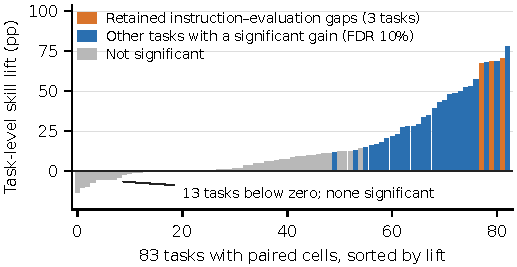
\includegraphics[width=\columnwidth]{figures/fig_task_lift.pdf}
\caption{Distribution of lift across the 83 tasks with paired cells. Significance comes from two-sided within-cell label permutation tests controlling the false discovery rate at 10\% across all 83 tasks.}
\label{fig:tasks}
\end{figure}

\subsection{How Many Negative Cells Would Pure Noise Produce?}
The same permutation null distribution also indicates the number of negative cells that would be obtained by chance if skills had no effect. Enumerate all the label assignments in each cell to get an expected 327.7 loss cells (central 95\% range 302-353) and 332.5 expected gain cells. According to the actual data, there are 169 loss cells and 547 gain cells; thus, the observed losses are significantly lower than the global zero-effect benchmark. The above inequality does not show that all skills are harmless; in fact, ``a combination of many beneficial skills and a few harmful skills'' would also result in total losses below 327.7, and it has not demonstrated that observing 169 negative cells is inherently harmful or shown how many of these cells represent actual regressions.

\subsection{Held-Out Trial Test}
To separate true effects from selection noise, we examine the 1,202 cells with at least two trials per condition. In each random split, we hold out one trial per condition, use the remaining decision trials to compute $r_{0}$, $r_{1}$, and $\Delta$, then test how the selected set of cells performs on its independent held-out trial pair. Point estimates are the average of 2,000 random divisions, the 95\% intervals are obtained by task-level resampling, and repeated divisions use the same underlying trial records without being independent replications.

Cells selected by high decision baseline ($r_{0}\ge0.8$, about 279 per split) have mean $\Delta=-16.1$\,pp on decision trials, but rebound to $-0.5$\,pp on held-out trial pairs (95\% interval $[-4.0,+3.1]$). This is textbook regression to the mean~\cite{barnett2005regression}: cells enter the $r_{0}\ge0.8$ group partly because their initial no-skill trials happened to succeed.

Cells selected by apparent loss on decision trials ($\Delta<0$, about 123 per split) average $-56.2$\,pp on decision trials, but $-9.9$\,pp on held-out trial pairs (95\% interval $[-16.8,-2.7]$), with 26\% showing losses and 18\% gains. As the mean of the hold-out set is still negative, apparent-loss cells are not truly random noise on average. Even so, the ratio $-9.9$ to $-56.2$\,pp should not be read directly as the fraction of real harm: the set contains different cells that exhibit different kinds of effects, each hold-out cell is based on one experiment on one side, and the observed data cannot tell apart the harm due to the skill itself from the interference between experiments in the same condition.

\subsection{Structural Features and Loss Rates}
Furthermore, we evaluate if having any of three characteristics of an audited skill package (different route of algorithm from reference solution, 3 tasks; containing placeholder directories, 4 tasks; containing license directories, 2 tasks) correlates with increased probability of having loss. Overall, the 9 tasks above do have a larger chance of loss than the other 74 tasks (20.9\% vs.\ 10.9\%), but they also have a much higher no-skill baseline (47.5\% vs.\ 28.2\%), so there is more room for loss to happen there: loss is only possible where the baseline is above zero. Restricting to positive-baseline cells ($r_{0}>0$), the gap narrows to 32.6\% (29/89) vs.~27.5\% (140/509), with a baseline-stratified Mantel--Haenszel odds ratio of 1.32 and a task-level bootstrap rate difference of $+5.1$\,pp (95\% interval $[-6.1,+18.5]$). Moreover, 13 of the 17 negative-lift tasks have none of these three structural features.

\subsection{Timeout Analysis}
In the second export, which records timeout status, the timeout rate is 8.99\% (219/2,436) for paired with-skill trials and 7.12\% (168/2,358) for no-skill trials, a ratio of 1.26 (95\% task bootstrap interval 1.03--1.56). Since we have not measured agent-interaction and computational steps, we state this small increase factually and without trying to explain its cause. When the same ratio is computed only for those cells that were chosen by $\Delta<0$, the ratio becomes 2.3 as an example of selection bias.

\section{Can a Gate Conditioned on Baseline Help?}
\label{sec:gate}
Given that the apparent losses are concentrated in high-baseline areas, it is natural to employ selective loading of skills; thus, only activate those skills that are anticipated to be beneficial. The three distinct outcomes of the above tests according to the three evaluation methods are presented.

\subsection{Gating Strategies}
\emph{Baseline cutoff:} load skills only when $r_{0}<0.8$. This demonstrates the most straightforward interpretation of ``retire skills if the bare model can perform adequately enough''; given that Wang et al.~\cite{wang2026beyondgain} use a threshold of 0.8 for scores obtained from a separate probe dataset, with the addition of a cross-model validity filter, our threshold rule is merely a rough approximation thereof.

\emph{Random-forest gate:} two random forests~\cite{breiman2001rf} use 17 features---$r_{0}$, an OpenHands harness indicator, and 15 static descriptors covering skill-package size, file composition, and lexical overlap with the prompt---to predict expected gain $\Delta$ and loss probability $P(\Delta<0)$, respectively. Each forest contains 25 trees with maximum depth 5, producing out-of-fold predictions via 10-fold cross-validation across cells. The max-gain version loads skills when $\hat{\Delta}>0.02$, while the risk-averse version loads when both $\hat{\Delta}>0$ and $\hat{P}(\Delta<0)<0.25$. The baseline-only forest uses only the first two features, with 20 trees of maximum depth 4.

\emph{Oracle-selector for Best-of-two:} directly selects the condition with the highest observed score.

\subsection{Three Evaluation Protocols}
\emph{Replay.} Standard offline log replay evaluates on the same recorded trials: when the policy loads skills, score $r_{1}$; when it declines, score $r_{0}$.

\emph{Permuted labels.} Within each cell, we randomly shuffle condition labels across trials, recompute $r_{0}$, $r_{1}$, $\Delta$, and loss indicators from the shuffled trials, refit the random forests, and perform offline replay. Given that shuffling inherently eliminates any skill effect, any positive effect or loss removal rate must be artificially created by the assessment process. Forest policies average 60 permutations; model-free rules average 2,000 permutations.

\emph{Held-out trial.} Cells with at least two trials per condition are restricted to; thus, 1,202 eligible cells remain and 219 are excluded. At each split, we randomly set aside one trial per condition solely for scoring, recalculate baseline features and training labels only from the rest of the decision trials, fit out-of-fold forests on these decision trials, and finally evaluate the load/skip decisions completely on the held-out trial pair. Gate thresholds and forest hyperparameters are set according to the configurations chosen in the previous full-data exploration and are not re-tuned. For each cell, we calculate the mean of held-out gains over random splits (60 for forests, 2,000 for other rules) and resample entire tasks 10,000 times to build the 95\% confidence intervals; due to the lack of internal refitting in bootstrap resampling and shared trial pools for splits, these intervals reflect task-sampling variation under a given fitted policy rather than independent replications.

\begin{table*}[t]
\caption{Gains (pp) Relative to ``Always Load Skills'' Under Three Evaluations}
\label{tab:gate}
\centering
\setlength{\tabcolsep}{5pt}
\begin{tabular}{@{}l r r r r r r@{}}
\toprule
 & \multicolumn{2}{c}{Replay} & \multicolumn{2}{c}{Permuted-label} & Decision-set & Held-out trial \\
\cmidrule(lr){2-3}\cmidrule(lr){4-5}
Strategy & Gain (95\% CI) & Removal rate & Gain & Removal & replay gain & gain (95\% CI) \\
\midrule
Baseline cutoff & +2.92 (+1.93, +4.02) & 43\% & +4.5 & 36\% & +3.7 & +0.12 ($-$0.67, +0.93) \\
RF gate, max gain & +2.95 (+1.95, +4.06) & 59\% & +6.5 & 82\% & +4.0 & $-$0.01 ($-$0.85, +0.87) \\
RF gate, risk averse & +2.12 (+1.03, +3.27) & 85\% & +5.7 & 94\% & +3.7 & $-$0.33 ($-$1.26, +0.65) \\
RF gate, baseline only & +0.72 ($-$0.97, +2.35) & 94\% & +5.5 & 94\% & +2.6 & $-$1.20 ($-$2.47, +0.09) \\
Best of two & +5.24 (+3.92, +6.63) & 100\% & +9.7 & 100\% & +5.8 & $-$1.61 ($-$3.01, $-$0.16) \\
\bottomrule
\end{tabular}\\[2pt]
\parbox{0.8\textwidth}{\footnotesize ``Removal'' refers to the proportion of cells with $\Delta<0$ where the strategy does not load skills. The permuted-label column is the mean over permutations; intervals are 95\% task bootstrap intervals.}
\end{table*}

\begin{figure}[t]
\centering
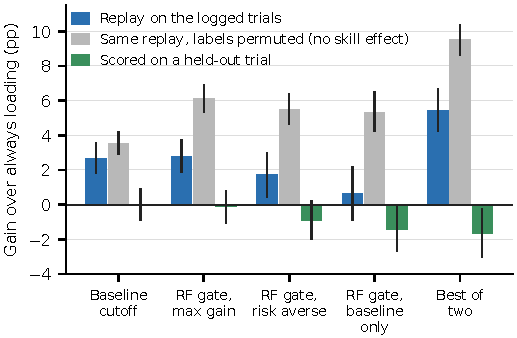
\includegraphics[width=0.82\columnwidth]{figures/fig_gate_eval.pdf}
\caption{Comparison of the three evaluation approaches outlined in Table~\ref{tab:gate}. The error bars for log replay and holdout trials represent 95\% task bootstrapped intervals, while those for permuted-label replay cover the 95\% central range of permutation results.}
\label{fig:gate}
\end{figure}

\subsection{Evaluation Results}
Table~\ref{tab:gate} and Figure~\ref{fig:gate} present the comparison of the three evaluation methods. Baseline cutoff and the two 17-feature forests in standard log replay are 2-3\,pp better than always-loading skills, and the risk-averse forest has eliminated 85\% of the negative cells. However, on label-shuffled data without a real skill effect, the same three strategies achieved an even higher gain of 4.5-6.5\,pp, and the risk-averse gate also eliminated 94\% of the ``loss'' cells. After scoring in held-out trials, none of the strategies achieved a statistically significant improvement; the confidence intervals for the baseline cutoff and both full-feature forests crossed zero with upper bounds below 1\,pp, well short of the 2-3\,pp claimed by log replay\cut{ (though the intervals are too wide to confirm that the actual effect is exactly zero)}. Choosing the decision-trial winner (Best of two) actually loses 1.61\,pp out of sample due to skipping cells that tie in decision trials but benefit from skills on held-out trial pairs.

The mechanism behind this illusion stems directly from $r_{0}$ entering three places simultaneously. Estimated from at most three trials, $r_{0}$ serves as a gate input feature, forms the negative half of the training target $\Delta=r_{1}-r_{0}$, and directly provides the fallback score when the gate skips loading. As a result, any cell whose no-skill trials happen to succeed is labeled ``high risk'', and those lucky passes are immediately credited to the policy. A simple calculation shows the magnitude: suppose a cell has true pass probability 0.7 both with and without skills (i.e., skills have no effect). With three no-skill trials, the probability all three pass is $0.7\times0.7\times0.7=0.34$; whenever this happens, the cutoff rule skips skills and records a score of 1.0 (while always-loading has expected score 0.7), creating about $+10$\,pp of gain on that cell from pure noise. In statistical terms, offline replay selects on a noisy baseline measurement and evaluates on the exact same random realization~\cite{cawley2010overfitting}, causing target leakage through a shared term~\cite{kapoor2022leakage}. Cross-validation across cells cannot remove this bias because the coupling occurs within each individual cell.

\subsection{What the Detector Actually Detects}
At first glance, the risk forest's ROC-AUC of 0.878 for predicting $\Delta<0$ seems to show strong ability to identify harmful skill packages. Table~\ref{tab:auc} decomposes this number and reveals a different picture. Checking only the binary indicator $r_{0}>0$ already yields AUC 0.829, because it directly excludes the 58\% of zero-baseline cells where loss is arithmetically impossible. Within the $r_{0}>0$ subset where losses can actually occur, the 17-feature forest reaches 0.65 under cell-level cross-validation but drops to 0.52 when holding out entire tasks. As the 15 static descriptors are the same for all cells in the same task, cell-level folds have used them as an implicit ``task ID'' for the forest. With folds grouped by task, the 17-feature forest exceeded the baseline-and-harness forest by 0.009 $\pm$ 0.009 AUC across all cells and by 0.026 $\pm$ 0.026 among cells with $r_{0}>0$. These values are the mean and standard deviation of the paired differences across eight random seeds. The forests also differed in size and depth (25 depth-5 trees versus 20 depth-4 trees), so the comparison cannot isolate the contribution of the additional features. Tellingly, the full-feature forest still achieves AUC 0.847 on label-shuffled data; when predicting the sign of $\Delta$ on held-out trials, it scores 0.70, only slightly ahead of the 0.67 obtained by the decision-trial indicator $r_{0}>0$ alone.

\begin{table}[t]
\caption{AUC for Predicting Loss ($\Delta<0$)}
\label{tab:auc}
\centering
\begin{tabular}{@{}lcc@{}}
\toprule
Predictor & All cells & Cells with $r_{0}>0$ \\
\midrule
Indicator $r_{0}>0$ & 0.829 & 0.500 \\
Numeric $r_{0}$ & 0.820 & 0.475 \\
\multicolumn{3}{@{}l}{\textbf{Folds over cells}} \\
Random forest (baseline + harness) & $0.833\pm0.005$ & $0.511\pm0.016$ \\
Random forest (all 17 features) & $0.879\pm0.005$ & $0.646\pm0.015$ \\
\multicolumn{3}{@{}l}{\textbf{Folds over tasks}} \\
Random forest (baseline + harness) & $0.828\pm0.004$ & $0.498\pm0.012$ \\
Random forest (all 17 features) & $0.837\pm0.009$ & $0.524\pm0.027$ \\
\bottomrule
\end{tabular}\\[2pt]
\parbox{\columnwidth}{\footnotesize Forest rows are mean $\pm$ standard deviation across 8 random seeds; standard deviation reflects fitting-process fluctuation, not sampling uncertainty.}
\end{table}

\section{Discussion}
\label{sec:discussion}
\textbf{What does skill lift actually measure.} The above three components of aggregate skill lift in this snapshot are: procedural guidance that effectively aids agents in task-solving, undeclared grading conventions communicated to the agent solely via the skill package, and variations in the ``no-skill'' baseline content among harnesses. Only the first one is the goal that a skill benchmark seeks to assess. The three gap tasks in our audit description account for approximately 18\% of the total lift; however, to determine how much of this increase is directly due to the missing prompt details, we would need to re-run the agents with patched instructions.

\textbf{Recommendations for benchmark maintainers.} (1) list all the grading rules applied by the grader in the task prompt, or explicitly tag tasks with required skill specifications and list them separately; although automatic comparison of grader constants, API calls and \code{task.md} can identify candidate tasks, full execution-path inspection and controlled runs are still needed for verification. (2) Extend the continuous-integration checks of skill packages to also scan for code-generator placeholders and non-skill directories in addition to frontmatter validation. (3) save all the skill directories that are actually shown in each test and maintain a constant set of non-task skills for the control groups. (4) Report task-level uncertainty intervals and plan for adequate trial funding. Roughly speaking, assuming independent binary success/failure trials at a moderate pass rate for the 18 configurations and an uncorrected one-sided 5\% test, three trials per condition yield a task-lift standard error of approximately 10\,pp; thus, a true loss exceeding about 24\,pp is needed for detection with 80\% power. Increasing to ten trials per condition reduces this detectable threshold to around 13\,pp.\cut{ The above are only for sample-size planning and do not provide exact guarantees.}

\textbf{Recommendations for methods that act on gains.} Any decisions based solely on cell-level differences derived from just three experiments will not be reliable enough to retire a skill or gate it. To evaluate a selective-loading policy, score its decisions on trials withheld from fitting and decision-making within each split. Repeat the same analysis after shuffling condition labels within each cell to check for apparent gains under the null. To assess generalization to unseen tasks, assign all configuration--task cells from the same task to the same fold. Likewise, loss-detection AUC should be reported within the $r_{0}>0$ subset where losses can actually occur.

\section{Threats to Validity}
\textbf{Snapshot differences.} Frozen snapshot is different from the final subset reported in the benchmark paper; it contains more configurations (some only cover a portion of the task set) and 11\% of the raw rows lack finite scores. Additionally, the two exports have different upstream filtering rules; the retrospective first archive saves only non-timeout trials with early logs, and the second export saves timeout trials. Therefore, the exact loss counts and task rankings of the final benchmark data may differ due to these reasons, and any differences between the two exports should not be attributed solely to time passing or model-capability changes. Although there are only about three experiments per cell per condition for sampling noise, the main cause of this noise is the same in the final data; however, the degree of noise varies according to pass rates and within-cell correlation.

\textbf{Held-out scoring variance.} Held-out evaluation scores decisions with only a single-trial pair per cell and excludes 219 low-trial-count cells.\cut{ Due to the noise of a single split, we average over repeated splits (60 for forests, 2,000 for other rules) and bootstrap-resample across tasks; however, repeated splits reuse the same trials instead of providing new replications, and bootstrap intervals do not account for variation due to refitting forests on new task samples.} Finally, intervals-crossing-zero only bound the strategy's gain and do not prove that it is exactly zero, as we did not specify an equivalence margin.

\textbf{Within-cell trial dependence.} Within-cell label permutation assumes trials under a given cell are exchangeable under the null. If there is correlated trial interference---for example, transient API or container failures affecting multiple trials in one condition---exchangeability is violated, and $p$-values or intervals may be skewed in either direction.

\textbf{Audit coverage.} The scope of our source audit is limited; two retained gap tasks are supported by controlled grader experiments, \task{flood-risk-analysis} is based on source-code review, and the earlier candidate tasks (\task{weighted-gdp-calc} and \task{sec-financial-report}) have not been verified.\cut{ As we have not conducted new-agent trajectory experiments, we cannot determine the amount of lift that would be retained when prompts specify grading rules.}\cut{ OpenHands directory and leak counts are also based on maintainer-reviewed exports instead of re-extraction from raw trajectories.}

\textbf{Retrospective policy setting.} After observing the run results, skill-package structural markers were coded; then, in an earlier analysis phase when all trials (including later held-out trial pairs) were visible, forest hyperparameters and gate thresholds were selected and fixed. Therefore, our hold-out protocol is a retrospective robustness test of a pre-defined fixed policy, not a prospective experiment on untouched new data; we conducted no secondary tuning, and thus do not rule out the possibility of training an effective gate with an independent probe set.

\section{Related Work}
Li et al.~\cite{li2026skillsbench} introduced the paired with/without-skill evaluation benchmark for coding agents in SkillsBench and recorded cross-harness variation and task-level declines; this paper provides a source-level grading audit and a statistical noise analysis of these declines. Wang and others~\cite{wang2026beyondgain}, who have done the most related work, have shown that raw gain scores are mixed up with baseline capability and proposed retiring skills by using dedicated bare-model probes; our held-out evaluation supports their warning and additionally demonstrates that baseline coupling distorts offline gating replay. Concurrent work has also studied skill compression~\cite{gao2026skillreducer}, skill routing and representation~\cite{liu2026implicitrouting,sun2026skillrep}, test-sufficiency criteria~\cite{tan2026skillcoverage}, evolutionary skill optimisation~\cite{ma2026skillneo} and safety oversight instructions~\cite{sanko2026oversight}.

More generally, in code generation~\cite{liu2023evalplus}, repository issue fixing~\cite{jimenez2024swebench,chowdhury2024swebenchverified}, question answering~\cite{gema2025mmluredux}, and even standard classification datasets~\cite{northcutt2021pervasive}, post hoc source audits have repeatedly altered the interpretation of top-tier benchmarks. Recent methodological checklists for agent benchmarks have focused on both task validity and outcome validity~\cite{kapoor2024agents,zhu2025abc}, and enforcing grading rules that are not in the task prompt directly violates task validity. Based on the above three well-known mechanisms: regression to the mean~\cite{barnett2005regression}, selection bias in model evaluation~\cite{cawley2010overfitting}, and target leakage via shared variables~\cite{kapoor2022leakage}, we present a study at the statistical level.

\section{Conclusion}
Several of the largest skill gains in this SkillsBench snapshot occur on tasks with instruction-evaluation gaps, as shown by two controlled grader tests and one source-level definition gap. Conversely, the occurrence of negative cells is no more frequent than that of trial noise alone in at most three trials per condition; thus, raw loss counts do not indicate that skills are detrimental, and after pooling data and correcting for multiple testing, no task shows a statistically significant loss. A gating strategy conditioned on the noisy no-skill baseline seems effective in naive log replay but does not show a statistically significant improvement in independent held-out trials. Although the above conclusions are only for the fixed policies and frozen snapshots analyzed here, they do not prove that skills are universally harmless or deny the principled feasibility of gating; however, they do suggest some clear methodological improvements: skill benchmarks should fully declare grader-enforced conventions in prompts and report uncertainty intervals, and any method that acts on observed skill gains should be validated with held-out trials and label-shuffled null distributions.

\section*{Data Availability}
Repository at \url{https://github.com/rrrrr4788/skillsbench-lift-reanalysis} has standardised trial and cell tables with per-row exclusion reasons, the source audit ledger, proposed prompt patches for the three tasks in Table~\ref{tab:contracts}, controlled grader check scripts, static checkers for generator placeholders and non-skill directories, and the whole reanalysis pipeline.\cut{ All tables and figures in this paper are directly reproducible from the above materials, and each output file contains the random seed, package versions, and input hashes; the held-out evaluation records the exact trial IDs held out in each split.}

\section*{Acknowledgment}
The authors have written the manuscript. No content of the final manuscript was created or modified by generative AI.

\bibliographystyle{IEEEtran}
\bibliography{IEEEabrv,refs}

\end{document}
